\chapter{Introduction}
\label{sec:introduction}
\bigskip

\section{Motivation}
\label{sec:introduction:motivation}

The thermal properties of snow are of interest to scientists studying Arctic and
sub-Arctic climates because, during the long, cold winters in this region,
snow's thermal behavior plays a critical role in determining the net energy
balance between Earth's surface and the atmosphere. After all, any heat transfer
occurring between the Earth and the atmosphere over snow-covered ground must go
through the snow first (Figure \ref{fig:climate}). In fact, the snow
itself may store and release energy over time.

\begin{figure}[h]
\centering
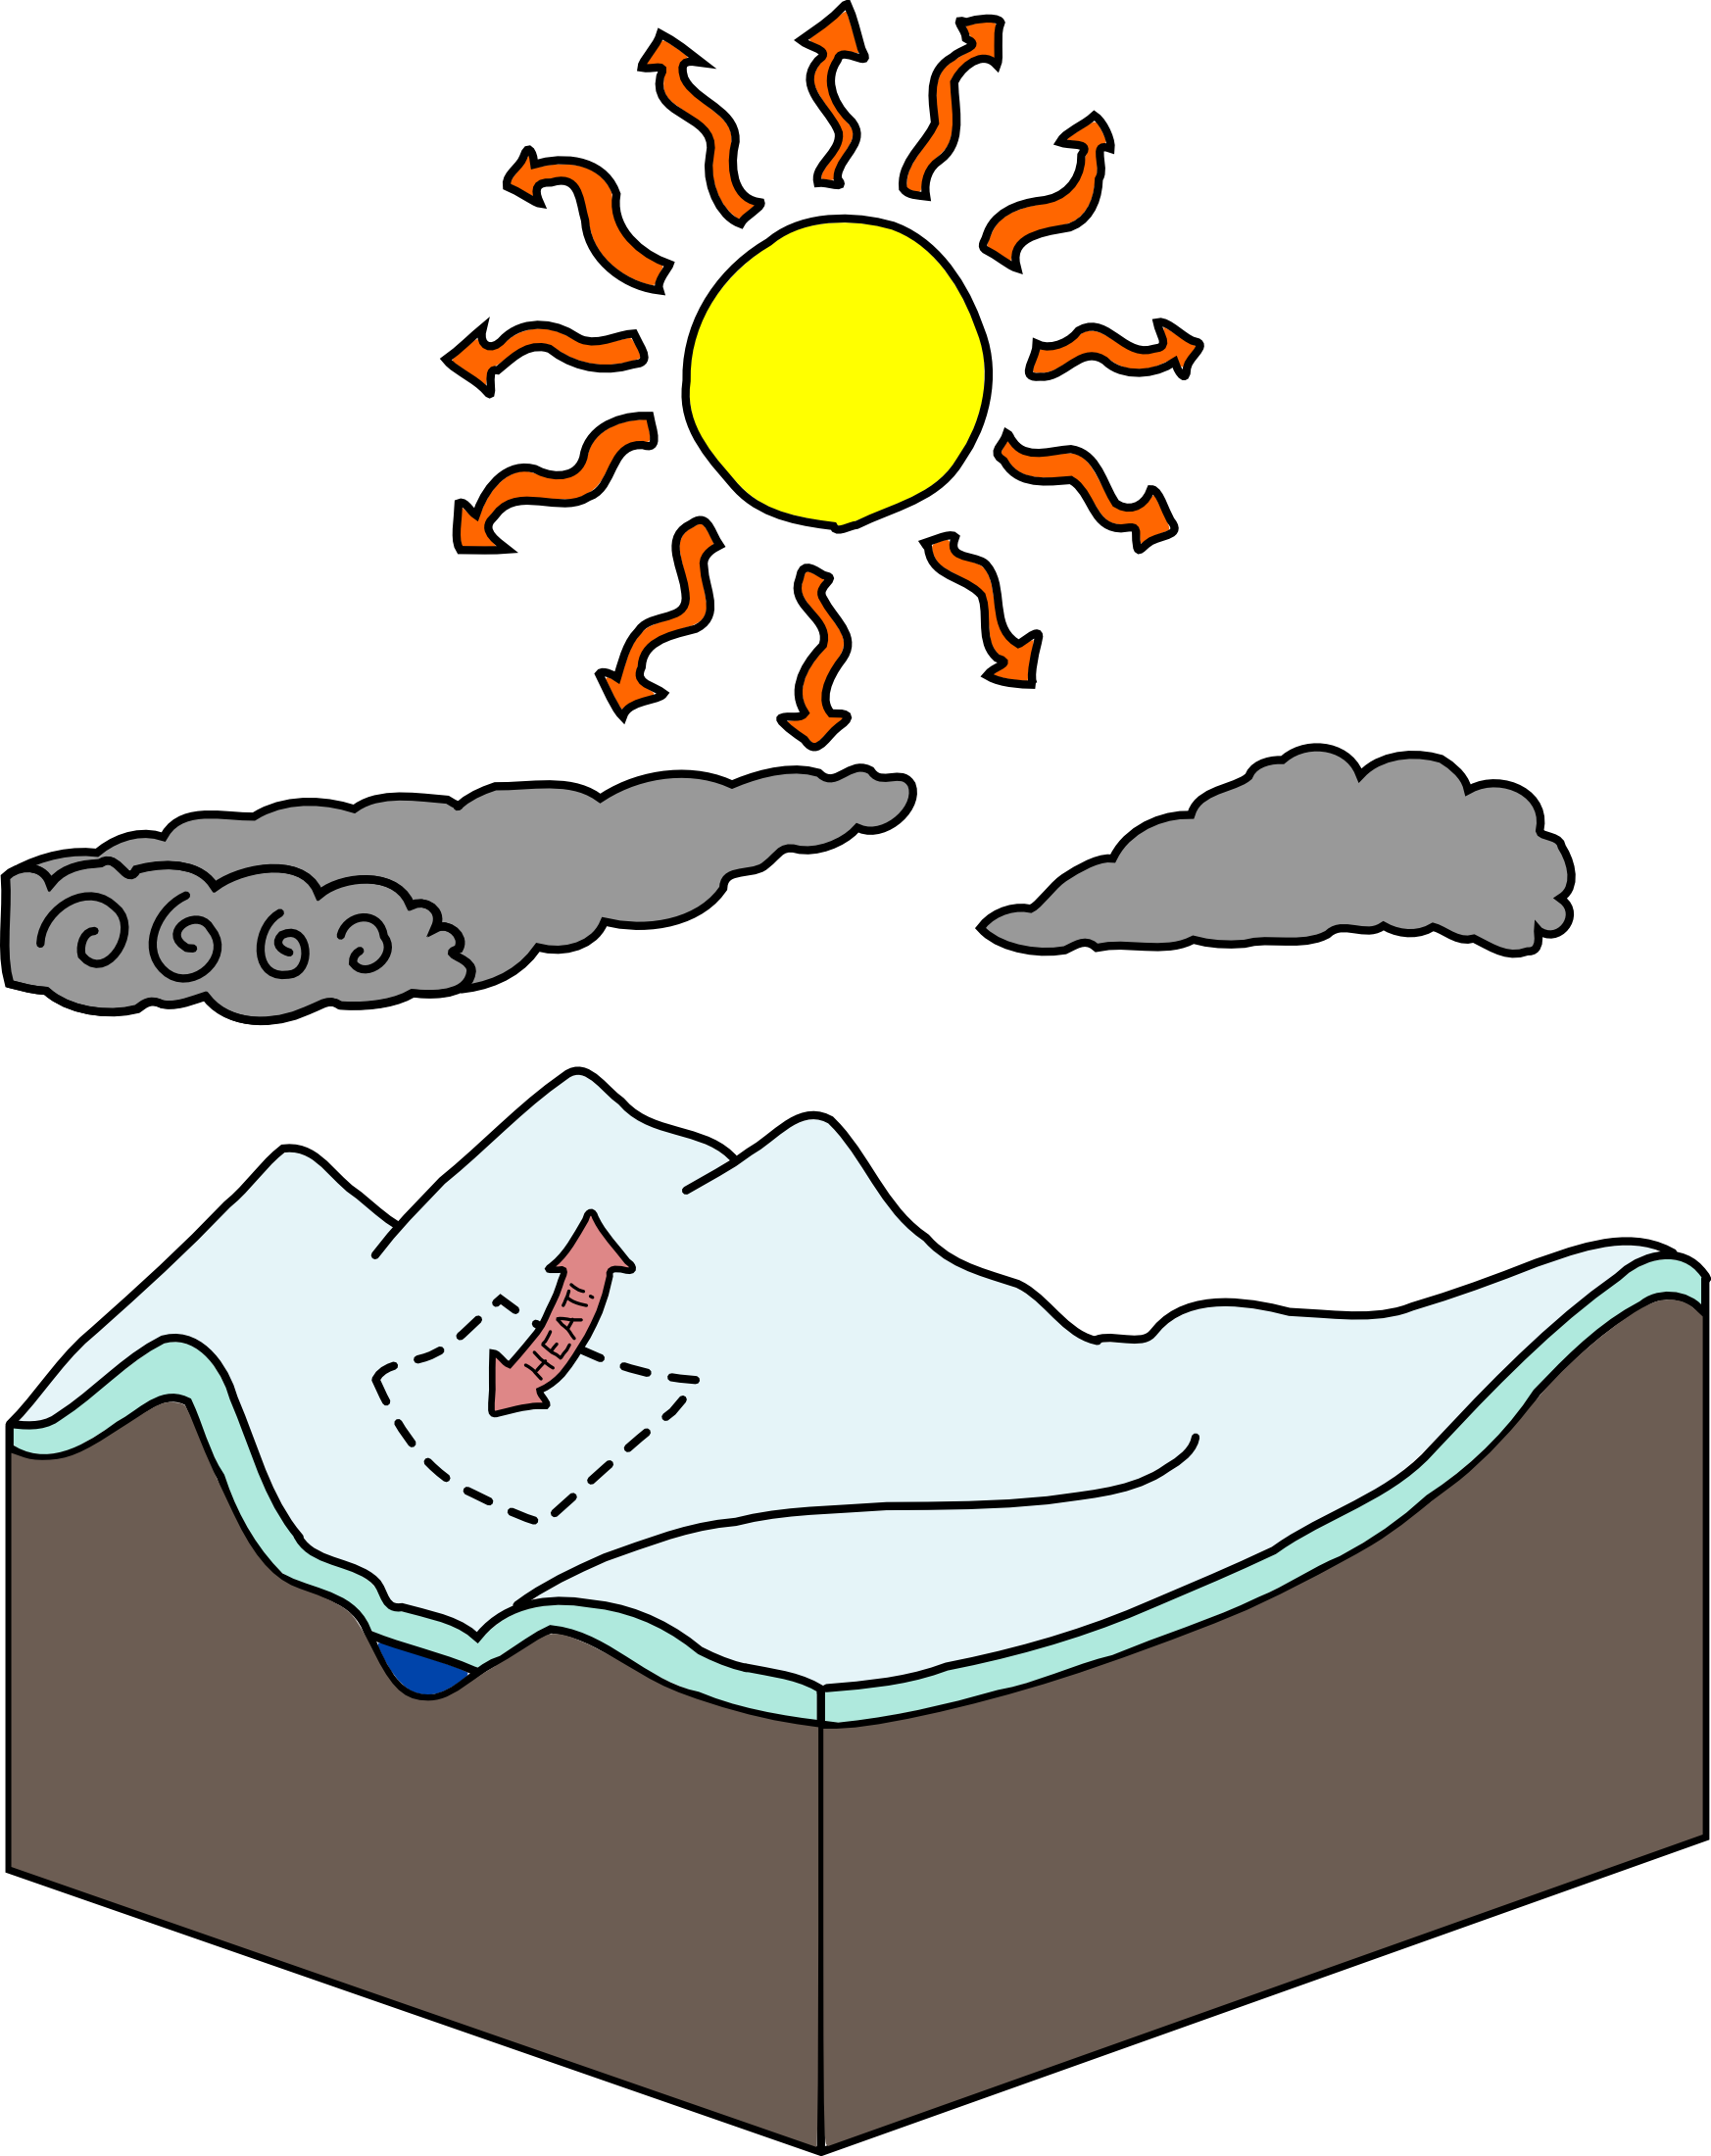
\includegraphics[width=0.4\textwidth]{fig/climate.png}
\caption{Arctic and Sub-Arctic climate is affected largely by heat transfer
between the atmosphere and the ground. Snowpack adds thermal resistance
transfer, affecting this heat transfer.}
\label{fig:climate}
\end{figure}

This energy transfer is critical in accurate climate models for these cold
regions, therefore the effective thermal conductivity of snow is a very
important factor for these models, and has been studied thoroughly. \cite{sturm1, sturm2, sturm3}


\section{Needle Probes: Basic Principles}
\label{sec:introduction:needles}

A more typical technique for measuring thermal conductivity, especially in the
context of engineering materials such as building insulation, is the guarded
hot plate. For this technique, a constant temperature gradient is induced across
the material, and heat flux over the material is measured.  By Fourier's Law,
\(k = \frac{\dot{q}l}{A\Delta T}\), where \(\dot{q}\) is the heat flux, \(A\) is
the cross-sectional area of the sample, \(l\) is the sample thickness, and 
\(\Delta T\) is the temperature difference across the sample. This technique
works well in many cases.

Another technique used for porous materials, such as soils and snow, is the
needle probe method. A needle probe consists of a long, thin needle with heating
wire running along its interior, and a temperature sensor in the center. This
configuration approximates an infinite line of constant-flux heat source
(Figure \ref{fig:needle_xsect}). \cite{basictheory}

\begin{figure}[h]
\centering
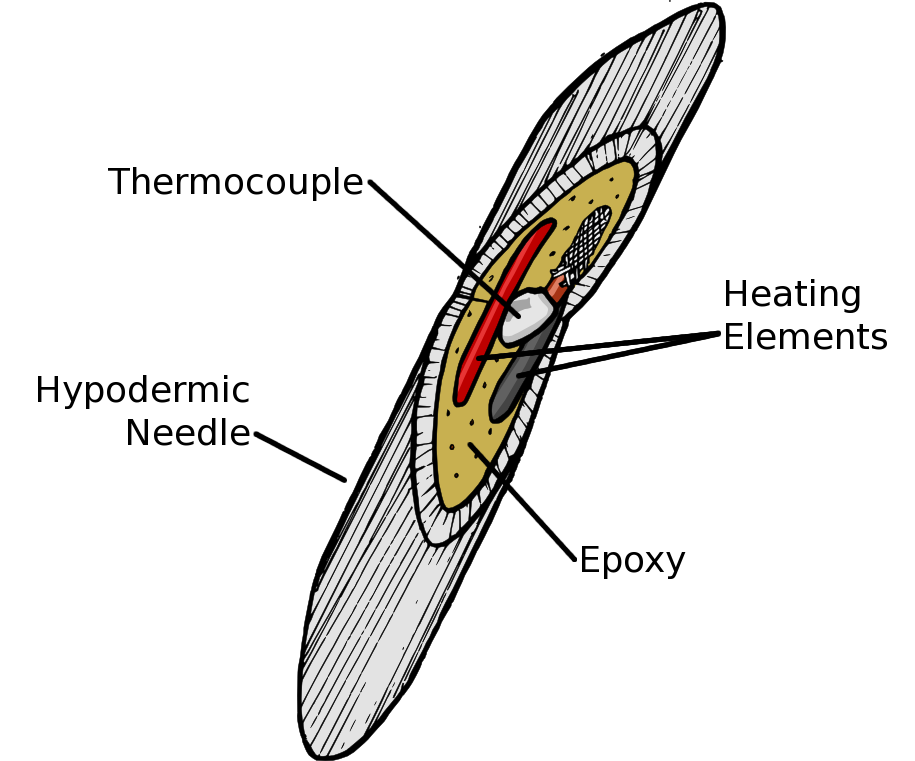
\includegraphics[width=0.4\textwidth]{fig/needle_xsect.png}
\caption{An illustration of a needle probe in cross-section. Note that the heat
trace in many needle probes, including the one used in experiments for this
research, actually wraps around an inner core instead of running axially through
the needle.}
\label{fig:needle_xsect}
\end{figure}

This needle is inserted into the material whose thermal conductivity is being
measured, and a constant voltage is applied to the needle's heating element.
This causes a constant heat flux along the needle, and, knowing the resistance
of the heat trace, this heat flux may be calculated. This causes the material's
temperature near the needle to rise (Figure \ref{fig:heating_curve}). After some
given amount of time, the heating element is turned off, and the temperature
around the needle begins to fall back towards ambient (Figure \ref{fig:cooling_curve}).


\begin{figure}[h]
\centering
\subfloat[Heating Curve]{
    \label{fig:heating_curve}
    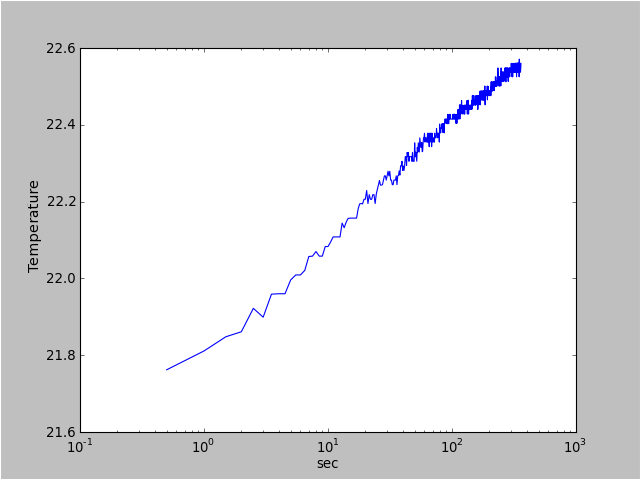
\includegraphics[width=0.4\textwidth]{fig/heating_curve.png}
}
\subfloat[Cooling Curve]{
    \label{fig:cooling_curve}
    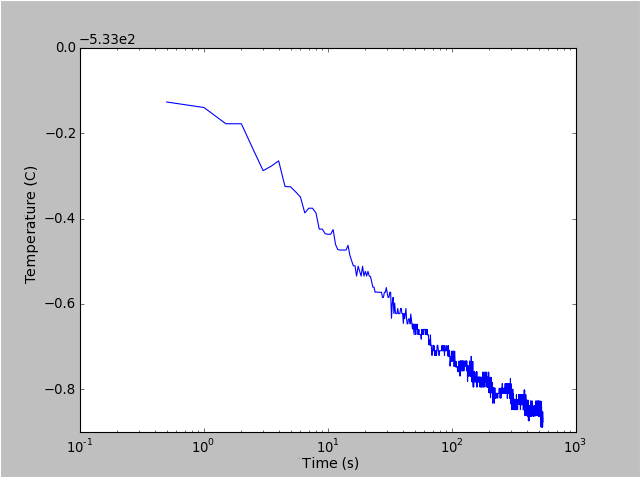
\includegraphics[width=0.4\textwidth]{fig/cooling_curve.png}
}
\caption{Typical heating and cooling curves from a needle probe measurement.
Time in the cooling curve is measured from the end of the heating curve.}
\end{figure}

The temperature data measured over time for these two periods are called the
heating cooling curves, respectively.  Based on the slopes of these
curves as a function of \(\ln(t)\) and approximate analytical solutions for
these situations, effective thermal conductivity may be calculated.

In this document, studies concentrate on the heating curve. In fact, the
numerical and analytical approaches focus exclusively on the heating curve. However, the
benchtop and in-situ measurements use both heating and cooling curves.

\section{Difficulties with the Needle Probe Method}

It should be noted that the needle probe method is not without its caveats. For
instance, it was shown that convection can and will occur in natural snowpack.
\cite{sturm3} In addition to the fact that convection in snowpack can change the
entire assumed heat transfer dynamic, heating the needle itself can cause this
convection to occur. This means that, when measurements are taken, there will
not only be ``transient'' regions due to short-term behavior, but also regions
where convection becomes a major force. Practically, this means that linear
portions (with respect to \(\ln(t)\)) must be found in between these regions
of instability.

\section{Snow Metamorphic Principles}
\label{sec:introduction:metamorphic}

The structure of a snowpack is strongly influenced by outside environmental
factors. Immediately after falling from the sky, snow begins to metamporphose as
it compacts under its own weight. In addition to this, temperature gradients
cause snow to sublimate and re-form in different regions of the snowpack, in a
process called vapor transport. Vapor transport is best known for causing
depth hoar, but occurs throughout the snowpack. Other events, such as
freeze-thaw events, may also change the form of snow. All these metamorphic
processes on snow cause it to form regions of varying thermal conductivity. In
some cases, these regions may form sharp, distinct layers with constant
properties, while in other cases they have continuously varying properties.

\section{Anisotropic Behavior in Snow}

Anisotropy in snow can occur in two ways: Either due to small-scale structure
in the snow, or due to macroscale features that cause anisotropy in the
aggregate.

On the small scale, snow may be anisotropic due to differences in grain boundary
connections, as illustrated in Figure \ref{fig:ex_structural}. \cite{pitman} In this case, the
layer of snow is itself anisotropic with respect to thermal conductivity because
grains connect to each other more completely in one direction than in another.
This occurs, for example, in depth hoar.

At a macroscale, alternating regions of low-conductivity and high-conductivity
material (isotropic or not) may also act in the aggregate as a single material of anisotropic thermal
conductivity---In other words, the effective thermal conductivity parallel to
the orientation of the layers may be different than the effective thermal
conductivity orthogonal to the layers. For example, suppose a composite exists of alternating layers, each of thickness
\(l\) and with conductivities \(k_1\) and \(k_2\), as in Figure
\ref{fig:ex_laminate}.

\begin{figure}[h]
\centering
\subfloat[Structural anisotropy, caused by differing inter-grain boundaries.]{
    \label{fig:ex_structural}
    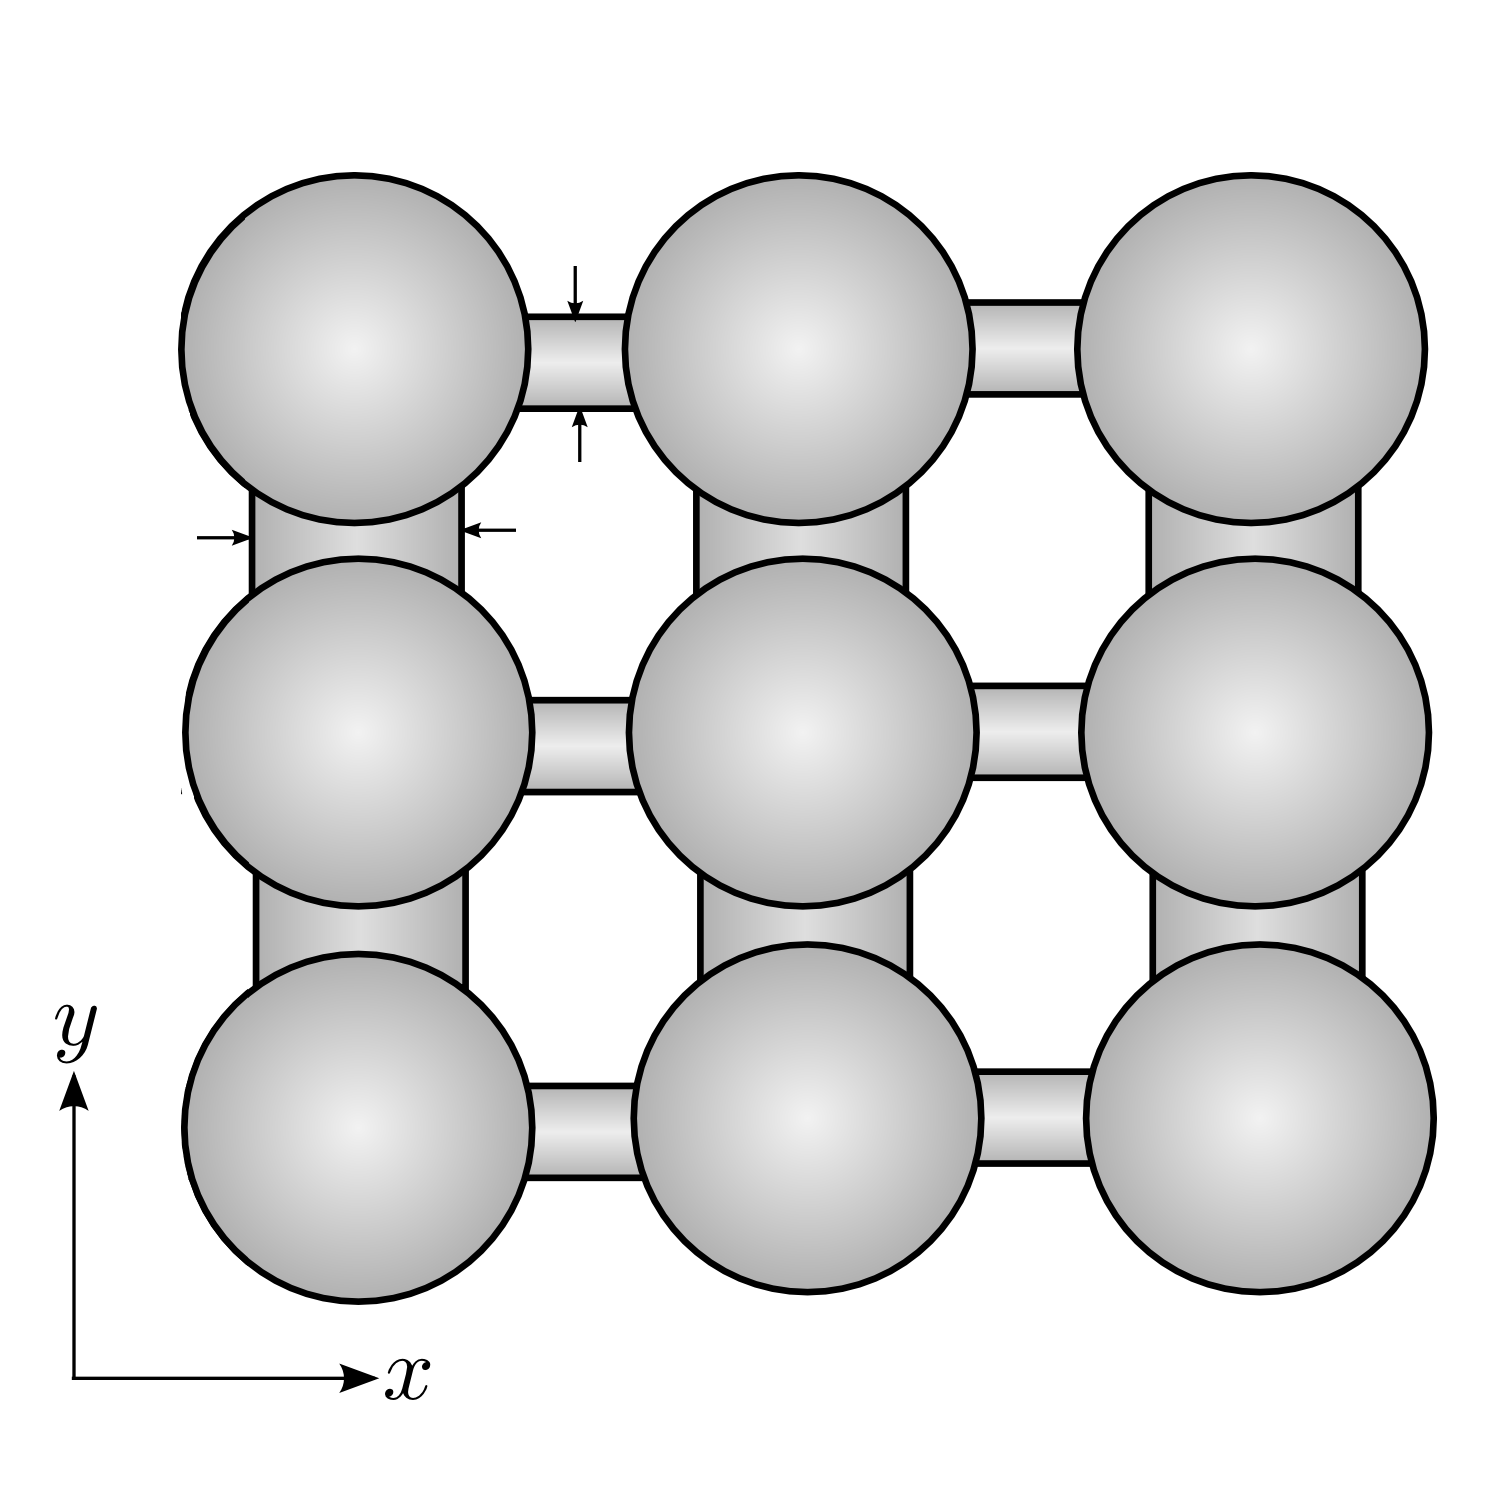
\includegraphics[width=0.4\textwidth]{fig/ex_structural.png}
}
\hspace{0.5in}
\subfloat[Aggregate anisotropy, caused by alternating layers of isotropic material.]{
    \label{fig:ex_laminate}
    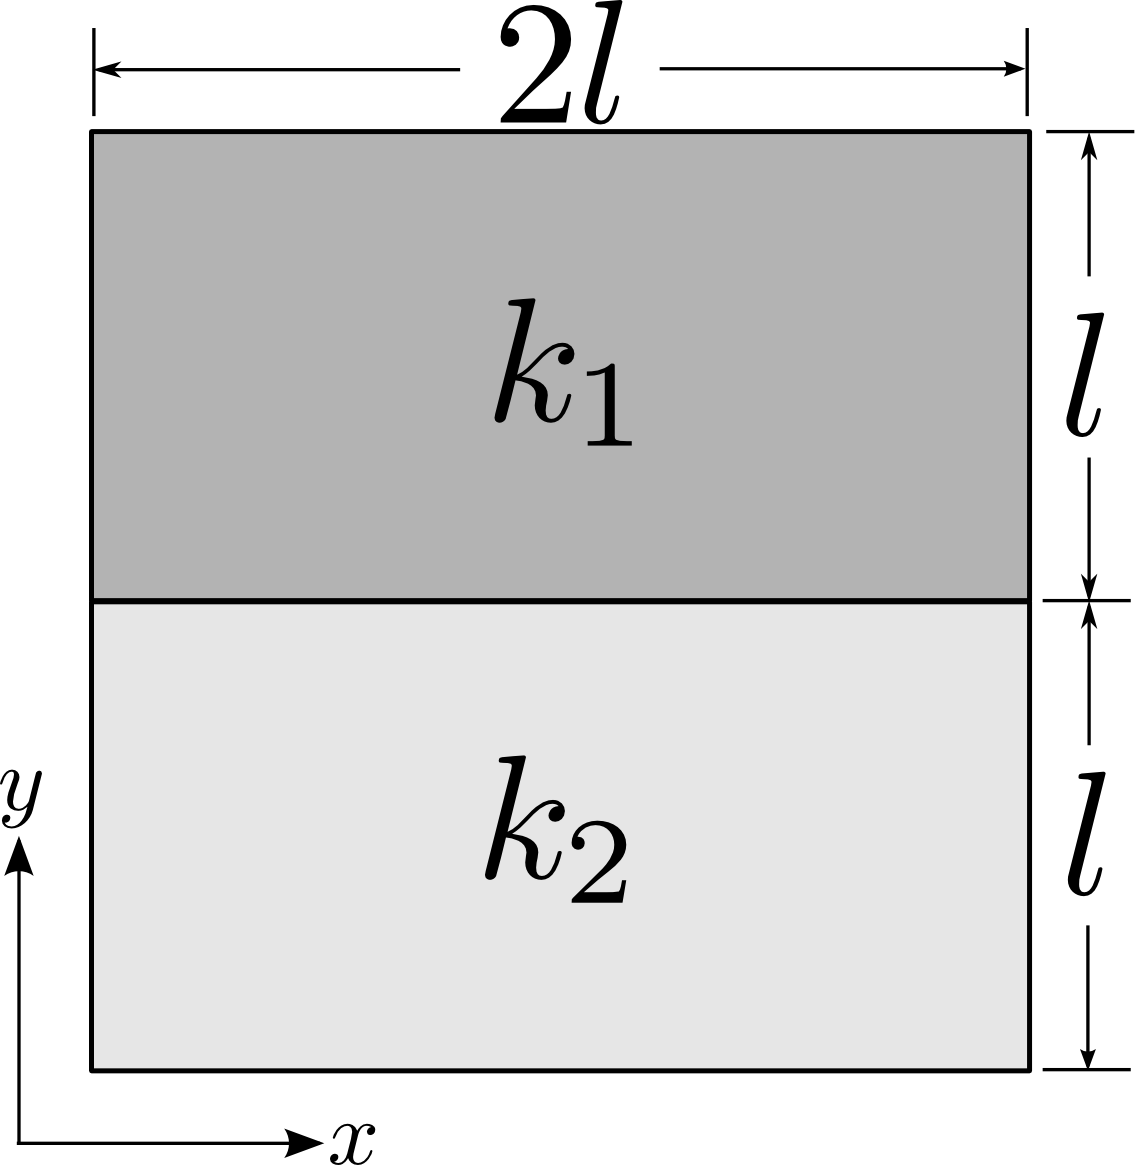
\includegraphics[width=0.4\textwidth]{fig/ex_laminate.png}
}
\caption{Anisotropy in snow may either occur as a result of microstructure features, or
in the aggregate due to geometry. }
\end{figure}

In the vertical direction, the effective thermal conductivity is
\(\frac12(k_1 + k_2)\) \cite{lunardini}. However, in the horizontal direction the effective
thermal conductivity is \(2\left( \frac1{k_1} + \frac1{k_2} \right)^{-1}\). An analogous analysis could be applied to a number of geometries.


\section{Measuring Anisotropic Thermal Conductivity}

Both structural and aggregate anisotropy raise a number of questions:

\begin{itemize}
\item Can anisotropic thermal conductivity in snow be measured with the needle
probe technique at all? If so, how accurately, and how many measurements would
one need?
\item How severe is anisotropy in snow? Is the amount of anisotropy
significant? Can horizontal measurements be used to approximate vertical thermal
conductivity?
\item Is anisotropy in snow predictable? That is, could one take a single
measurement and extrapolate from it the anisotropic thermal conductivity?
\item Can anisotropy in snow explain historical differences between various
thermal conductivity measurements of snow using both the guarded hot plate and
needle probe techniques?
\end{itemize}


%I can make conclusions/comments on most of these points.

This document primarily focuses on the first question. Developing a way
to measure anisotropic thermal conductivity with needle probes should enable
future researchers in answering the other questions. However, these other
questions will also, in part, be addressed.

\section{Anisotropic Model}

In every model studied, it has been assumed that the horizontal plane has the
same thermal conductivity and that only the vertical direction differs. In other
words, \(k_x = k_y = k_{xy} \ne k_z\). Each model aims to predict the effective
conductivity, \(k_{\textrm{eff}}\) as a function of angle.

In both analytical and numerical models and in the measurements, the angle
parameter, \(\theta\), is measured from the horizontal plane, as in Figure 
\ref{fig:angle}.

\begin{figure}[h]
\centering
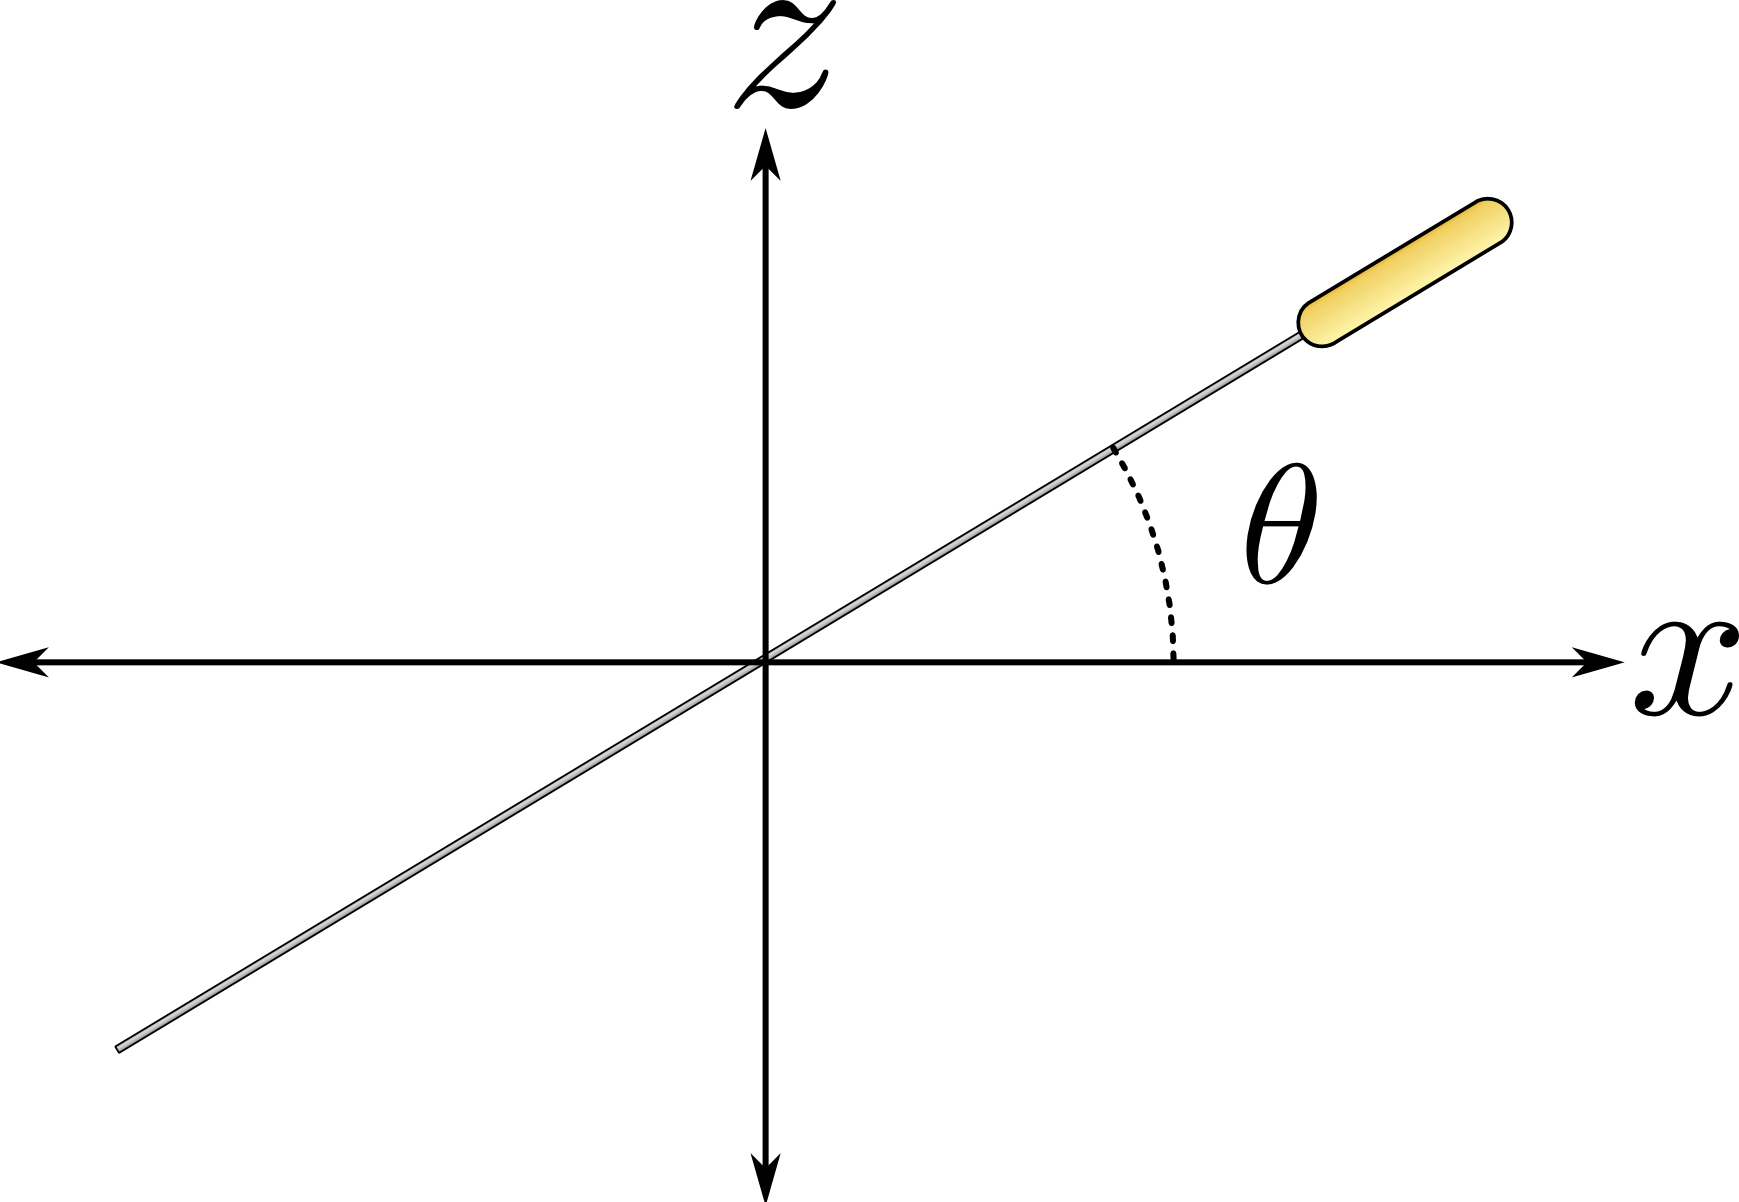
\includegraphics[width=0.3\textwidth]{fig/angle.png}
\caption{A diagram illustrating the measurement \(\theta\) in models and
measurements in this document. In all these cases, the angle is measured from
the horizontal plane, which is also the plane of isotropy. }
\label{fig:angle}
\end{figure}


\section{Document Outline}

First, this document will discuss the differential equations associated with
adapting the isotropic needle probe technique to the anisotropic case, as well
as analytical approaches to solving them. 

Second, the use of 3D finite element models in COMSOL with MATLAB to find 
numerical solutions to the problem will be discussed.

Then, this document will cover techniques for testing the predictions of the
these approaches with both real snow and engineered anisotropic materials, in
this case using table salt and table sugar.

The results of the analytical and numerical approaches will then be compared to
each other and the measurements of snow and engineered materials. The meanings
of these results are also discussed.

Finally, unanswered questions and avenues for future research
will be elucidated.
